%! Author = itgramic
%! Date = 24.11.23

% Preamble
\chapter{Einführung}
\begin{flushleft}
    Im Rahmen des von Microsoft indizierten Patchdays, bei dem Microsoft alle 2 Monate einen Patch veröffentlicht, müssen auch die \Gls{JBoss}-Server des KIS Phoenix angefasst werden.
    Die Server werden dabei von \Gls{Ivanti} mit den Patches betankt, so das man nur noch einen Reboot durchführen und nicht noch erst die Patches herunterladen muss..
\end{flushleft}
\begin{flushleft}
    Das KIS Phoenix verfügt dabei über 4 JBoss-Server, 2 für die Testsysteme resp.
    das Demosytsem und 2 für das produktive System.
    \begin{figure}[H]
        \centering
        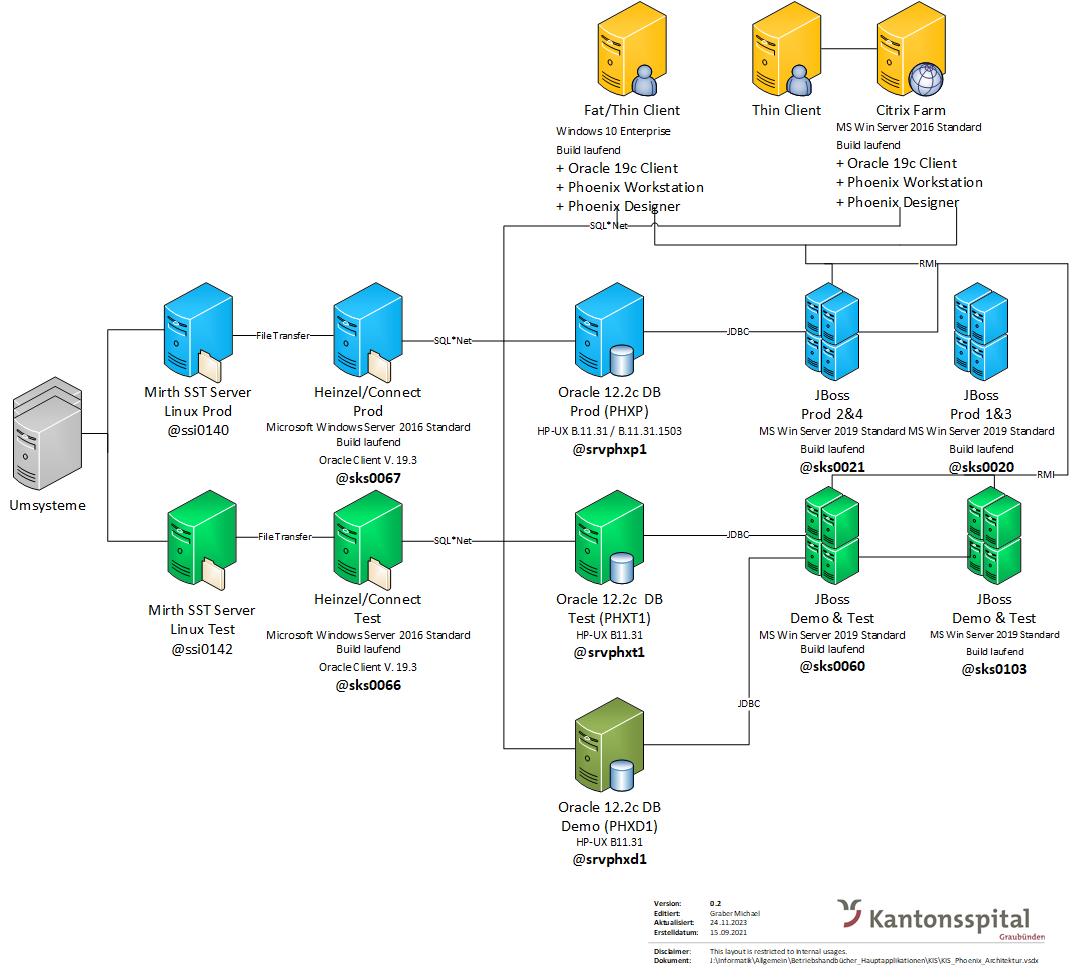
\includegraphics[width=1\linewidth]{source/introduction/KIS_Phoenix_Architektur}
        \caption{Architektur KIS Phoenix\cite{KFDFYH5H}}
        \label{fig:architektur-kis-phoenix}
    \end{figure}
\end{flushleft}
\begin{flushleft}
    Das Test1 und Demosystem hat je einen JBoss-Node auf einer Seite, das Test2 hat nur einen Node auf einem Server.
    Das Produktivsystem hat je Site zwei Nodes, also insgesamt vier Nodes.
\end{flushleft}
\begin{flushleft}
    Die Verzeichnisstruktur sieht dabei wie folgt aus:

%    \dirtree{%
%    .1 spam.
%    .2 ham.
%    .2 eggs.
%    .3 more spam.
%    .3 dead parrots.
%    }

%    \dirtree{%
%    .1 Laufwerk.
%    .2 {phoenix\_server\_system\_version}.
%    .3 node.
%    .4 standalone.
%    .5 log.
%    .6 server.log.
%    }

%    \dirtree{%
%
%    .1 spam.
%    .2 ham.
%    .2 eggs.
%    .3 more spam.
%    .3 dead parrots.
%%    .4 potatoes.
%    }

    \dirtree{%
        .1 /.
        .2 laufwerk.
        .3 phoenix-server-<system>-<version>.
        .4 <node>.
        .5 standalone.
        .6 log.
        .7 server.log.
    }

    \begin{mdframed}
    Meistens existieren pro Node die verzeichnisse meherer Versionen, üblicherweise immer die der aktuellen und vorangehenden Version.\\Daher aufpassen in welchem Verzeichnis man ist!
    \end{mdframed}

    Auf jedem Server wurde zudem \textit{baretail.exe} installiert, ein Logging-Tool welches eine Echtzeitüberwachung der Logs ermöglicht.
    Leider ist es nicht auf jedem Server gleich installiert sondern individuell.
\end{flushleft}
\begin{flushleft}
    Die genaue Konfiguration sieht wie folgt aus:
\end{flushleft}
%\begin{flushleft}
    % Please add the following required packages to your document preamble:
    % \usepackage{booktabs}
    % \usepackage{graphicx}
    % \usepackage{lscape}
% Please add the following required packages to your document preamble:
% \usepackage{graphicx}
% \usepackage{lscape}
% Please add the following required packages to your document preamble:
% \usepackage{graphicx}
% \usepackage{lscape}
\begin{landscape}
\begin{table}[]
\centering
\resizebox{\columnwidth}{!}{%
\begin{tabular}{lccccccccccc}
\hline
\textbf{Typ}                                                     & \textbf{Applikationsserver} & \textbf{}                & \textbf{}                & \textbf{}                & \multicolumn{5}{c}{}                                                                                                                      & \multicolumn{2}{c}{\textbf{Schnittstellenserver}} \\ \hline
\textbf{\begin{tabular}[c]{@{}l@{}}Systeme\\ Rolle\end{tabular}} & \multicolumn{2}{c}{\textbf{Produktion}}                & \multicolumn{2}{c}{\textbf{Produktion}}             & \multicolumn{5}{c}{\textbf{Test- und Demosystem Test- und Demosystem}}                                                                    & \textbf{Produktion}        & \textbf{Test}        \\ \hline
\multicolumn{1}{l|}{\textbf{Physikalischer Hostname}}            & \multicolumn{2}{c}{sks0020}                            & \multicolumn{2}{c}{sks0021}                         & \multicolumn{3}{c}{sks0060}                                                       & \multicolumn{2}{c}{sks0103}                           & sks0067                    & sks0066              \\
\multicolumn{1}{l|}{\textbf{IP Adresse phy. Host}}               & \multicolumn{2}{c}{10.0.22.43}                         & \multicolumn{2}{c}{10.0.22.44}                      & \multicolumn{3}{c}{10.0.22.52}                                                    & \multicolumn{2}{c}{10.0.22.15}                        & 10.0.22.54                 & 10.0.22.53           \\
\multicolumn{1}{l|}{\textbf{IP Submask}}                         & \multicolumn{11}{c}{255.255.255.0}                                                                                                                                                                                                                                                                           \\
\multicolumn{1}{l|}{\textbf{Gateway}}                            & \multicolumn{11}{c}{10.0.22.1}                                                                                                                                                                                                                                                                               \\
\multicolumn{1}{l|}{\textbf{DNS 1}}                              & \multicolumn{11}{c}{10.0.16.163}                                                                                                                                                                                                                                                                             \\
\multicolumn{1}{l|}{\textbf{DNS 2}}                              & \multicolumn{11}{c}{10.0.16.163}                                                                                                                                                                                                                                                                             \\
\multicolumn{1}{l|}{\textbf{Timeserver}}                         & \multicolumn{11}{c}{10.10.146.196}                                                                                                                                                                                                                                                                           \\
\multicolumn{1}{l|}{\textbf{JBoss Nodes}}                        & prod1                       & prod3                    & prod2                    & prod4                    & demo11                    & test11                    & test21                    & demo12                    & test12                    & \multicolumn{2}{c}{-}                             \\
\multicolumn{1}{l|}{\textbf{Windows Services}}                   & PhoenixJBossEAP\_prod\_1    & PhoenixJBossEAP\_prod\_3 & PhoenixJBossEAP\_prod\_2 & PhoenixJBossEAP\_prod\_4 & PhoenixJBossEAP\_demo1\_1 & PhoenixJBossEAP\_test1\_1 & PhoenixJBossEAP\_test2\_1 & PhoenixJBossEAP\_demo1\_2 & PhoenixJBossEAP\_test1\_2 & \multicolumn{2}{c}{-}                             \\ \hline
\end{tabular}%
}
\caption{Spezifikationen KIS Phoenix Applikations- und Schnittstellenserver}
\label{tab:kis-phoenix-server-specs}
\end{table}
\end{landscape}
%\end{flushleft}